\documentclass[10pt,a4paper]{article}
\usepackage{amsmath}
\usepackage{amssymb}
\usepackage{graphicx}
\usepackage{color}
\usepackage{fancyhdr}
\usepackage{fancyvrb}
\usepackage[margin=3.5cm]{geometry}
\usepackage{framed}
\usepackage{enumerate}
\usepackage{textcomp}
\def\ket#1{\left|#1\right\rangle}
\def\bra#1{\left\langle#1\right|}
\def\braket#1{\left\langle#1\right\rangle}

\definecolor{linkcol}{rgb}{0.0, 0.0, 0.5}
\usepackage[colorlinks=true,urlcolor=linkcol,citecolor=black,linkcolor=linkcol]{hyperref}

\setcounter{section}{0}
\renewcommand\thesection{\arabic{section}}
\renewcommand\thesubsection{\thesection.\arabic{subsection}}

\fancyhf{}
\lhead{\tiny Y.~D.~Chong (2018)}
\rhead{\scriptsize MH2801: Complex Methods for the Sciences}
\lfoot{}
\rfoot{\thepage}
\pagestyle{fancy}

\makeatletter
\def\PY@reset{\let\PY@it=\relax \let\PY@bf=\relax%
    \let\PY@ul=\relax \let\PY@tc=\relax%
    \let\PY@bc=\relax \let\PY@ff=\relax}
\def\PY@tok#1{\csname PY@tok@#1\endcsname}
\def\PY@toks#1+{\ifx\relax#1\empty\else%
    \PY@tok{#1}\expandafter\PY@toks\fi}
\def\PY@do#1{\PY@bc{\PY@tc{\PY@ul
\def\PYZdl{\char`\$}
\def\PYZhy{\char`\-}
\def\PYZsq{\char`\'}
\def\PYZdq{\char`\"}
\def\PYZti{\char`\~}

\begin{document}
\setcounter{page}{7}

\section{Derivatives}\label{derivatives}

 The \textbf{derivative} of a function $f$ is another function,
$f'$, defined as follows:
\begin{equation}
f'(x) \;\equiv\; \frac{df}{dx} \;\equiv\; \lim_{\delta x \rightarrow 0} \, \frac{f(x + \delta x) - f(x)}{\delta x}.
\end{equation}
This kind of expression is called a \textbf{limit expression} because it
involves a limit (in this case, the limit where $\delta x$ goes to
zero).

If the value of the above limit expression is unique and well-defined
within some domain of $x$, we say that the derivative ``exists'' in
that domain. We also say that $f(x)$ is \textbf{differentiable} in
that domain. It can be shown that a differentiable function is
automatically \href{00_mathfunctions.ipynb\#continuity}{continuous}.
If the derivative exists, we can define the second-order derivative of
$f$ as the derivative of $f'$. Third- and higher-order derivatives are
defined similarly.

\begin{figure}[h]
  \centering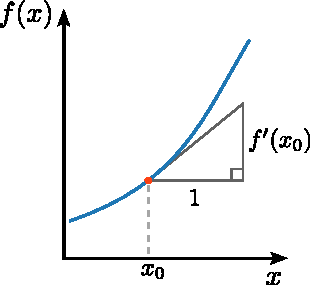
\includegraphics[width=0.32\textwidth]{derivative}
\end{figure}

The derivative represents the slope of the graph of $f(x)$, as shown
in the above figure.  The second derivative represents the curvature;
in the above figure, the curve is upward-curving, so the second
derivative is positive.

\subsection{Properties of derivatives}
\label{properties-of-derivatives}

\hypertarget{rules-for-limit-expressions}{%
\subsubsection{Rules for limit
expressions}\label{rules-for-limit-expressions}}

Since derivatives are defined using limit expressions, let us first
summarize the rules governing limits.

First, the limit of a linear superposition is equal to a linear
superposition of limits. This means that, given two constants $a_1$
and $a_2$ and two functions $f_1$ and $f_2$,
\begin{equation}
\lim_{x \rightarrow c} \big[a_1 \,f_1(x) \;+\; a_2\, f_2(x)\big] = a_1 \lim_{x \rightarrow c} f_1(x) \;+\; a_2 \lim_{x \rightarrow c} f_2(x).
\end{equation}
Second, limits obey a product rule and a quotient rule:
\begin{equation}
\begin{aligned}\lim_{x \rightarrow c} \big[\;f_1(x) \; f_2(x)\;\big] &= \Big[\lim_{x \rightarrow c} f_1(x)\Big]\;\Big[\lim_{x \rightarrow c} f_2(x)\Big]  \\ \lim_{x \rightarrow c} \left[\;\frac{f_1(x)}{f_2(x)}\;\right] &= \frac{\lim_{x \rightarrow c} f_1(x)}{\lim_{x \rightarrow c} f_2(x)}. \end{aligned}
\end{equation}
As a special exception, the product rule and quotient rule should be
ignored whenever they produce results of $0 \times \infty$,
$\infty/\infty$, or $0/0$, because such combinations are undefined.
For instance, naively applying the product rule to both of the following
limit expressions gives $0 \times \infty$, but their actual values are
zero and infinity:
\begin{equation}
\begin{aligned}\lim_{x \rightarrow 0}\Big[\,x^2\;\frac{1}{x}\;\Big] &= 0  \;\quad \ne\;\;\;\lim_{x \rightarrow 0}\Big[\,x^2\,\Big]\; \lim_{x \rightarrow 0}\Big[\,\frac{1}{x}\,\Big]\\ \lim_{x \rightarrow 0}\Big[\,x\;\frac{1}{x^2}\;\Big] &= \infty \quad \ne\;\;\;\lim_{x \rightarrow 0}\Big[\,x\,\Big]\; \lim_{x \rightarrow 0}\Big[\,\frac{1}{x^2}\,\Big].\end{aligned}
\end{equation}

\subsubsection{Composition rules for derivatives}
\label{composition-rules-for-derivatives}

Using the rules for limit expressions, we can derive the elementary
composition rules for derivatives:
\begin{equation}
\begin{aligned}\frac{d}{dx}\big[\,\alpha\, f(x) + \beta\, g(x)\,\big] &= \alpha\, f'(x) + \beta\, g'(x) \quad &\textrm{(linearity)}& \\   \frac{d}{dx}\big[\,f(x) \, g(x)\,\big] &= f(x) \, g'(x) + f'(x) \, g(x) &\textrm{(product}\;\textrm{rule)}& \\   \frac{d}{dx}\big[\,f(g(x))\,\big] &= f'(g(x)) \, g'(x) &\textrm{(chain}\;\textrm{rule)}&\end{aligned}
\end{equation}
These can all be proven by direct substitution into the definition of
the derivative, and taking appropriate orders of limits. With the aid of
these rules, we can prove various standard results, such as the ``power
rule'' for derivatives: \[\frac{d}{dx} \big[x^a\big] = a x^{a-1}.\]

The linearity of the derivative operation has the important
implication that derivatives ``commute'' with sums, i.e.~you can move
them to the left or right of summation signs. This fact can be used to
help prove that the exponential function is its own derivative:
\begin{equation}
  \frac{d}{dx} \left[\exp(x)\right] = \frac{d}{dx} \sum_{n=0}^\infty\frac{x^n}{n!} = \sum_{n=0}^\infty\frac{d}{dx} \, \frac{x^n}{n!} = \sum_{n=1}^\infty \frac{x^{n-1}}{(n-1)!} =\exp(x)
\end{equation}

Derivatives also ``commute'' with limits. For example, we can use this
on the alternative definition of the exponential function:
\begin{align}
  \begin{aligned}
  \frac{d}{dx} \left[\exp(x)\right] &=
  \frac{d}{dx} \lim_{n\rightarrow\infty} \left(1+\frac{x}{n}\right)^n
  = \lim_{n\rightarrow\infty} \frac{d}{dx} \left(1+\frac{x}{n}\right)^n \\
  &= \lim_{n\rightarrow\infty} \left(1+\frac{x}{n}\right)^{n-1}
  \;= \exp(x)
  \end{aligned}
\end{align}

\subsection{Taylor series}

A function is \textbf{infinitely differentiable} at a point $x_0$ if
all orders of derivatives are well-defined (i.e., first derivative,
second derivative, etc.) at $x_0$. Not all functions behave this way:
for example, $f(x) = |x|$ has a first derivative which is
discontinuous at $x = 0$, which means that it has no well-defined
second derivative at that point.

If a function is infinitely differentiable at $x_0$, then near that
point it can be expanded in a \textbf{Taylor series}:
\begin{equation}
\begin{aligned}f(x) \;&=\; \sum_{n=0}^\infty \frac{(x-x_0)^n}{n!} \left[\frac{d^n}{dx^n} f\right](x_0) \\&=\; f(x_0) + (x-x_0)\, f'(x_0) + \frac{1}{2}\, (x-x_0)^2\, f''(x_0) + \cdots\end{aligned}
\end{equation}
Here, the ``zeroth derivative'' refers to the function itself.

The Taylor series can be derived by assuming that $f(x)$ can be
written out as a general polynomial involving terms of the form
$(x-x_0)^n$; using the definition of the derivative, we can derive the
polynomial coefficients appearing in the series. Because this polynomial
approximation is only an assumption, there is no guarantee that the
Taylor series actually converges to the true value for a given value of
$x \ne x_0$. For many functions, the Taylor series converges only if
$|x-x_0|$ is smaller than a certain amount.

\pagebreak
Here is a list of useful Taylor series:

\begin{align}
  \frac{1}{1-x} = 1 + x + x^2 + x^3 + \cdots\mathrm{for} \; |x| < 1 \\
  \ln(1-x) = -x - \frac{x^2}{2} - \frac{x^3}{3} - \frac{x^4}{4} - \cdots \quad \mathrm{for} \; |x| < 1 \\
  \sin(x) = x - \frac{x^3}{3!} + \frac{x^5}{5!} - \frac{x^7}{7!} + \cdots \\
  \sinh(x) = x + \frac{x^3}{3!} + \frac{x^5}{5!} + \frac{x^7}{7!} + \cdots \\
  \cos(x) = 1 - \frac{x^2}{2!} + \frac{x^4}{4!} - \frac{x^6}{6!} + \cdots \\
  \cosh(x) = 1 + \frac{x^2}{2!} + \frac{x^4}{4!} + \frac{x^6}{6!} + \cdots
\end{align}
Apart from the first row, the others are actually exact for all $x$.
The sine/cosine functions and hyperbolic functions are ``entire'',
which means that their Taylor series converge everywhere in
$\mathbb{R}$. If you pick a large value of $x$, however, you may have
to sum to a very high order before the series converges to an accurate
value.

\subsection{Ordinary differential equations}
\label{ordinary-differential-equations}

A differential equation is an equation involving several different
derivatives of a function. For example,
\begin{equation}
\frac{df}{dx} = \kappa\, f(x)
\end{equation}
is a differential equation involving both $f$ and its first
derivative. Specifically, this is called an \textbf{ordinary
  differential equation}, because $f$ is a function involving a single
variable $x$, rather than multiple variables.

Finding a solution for the differential equation means finding a
function that satisfies the equation. There is no single method for
solving differential equations. In some cases, we can guess the
solution; for example, by trying different elementary functions, we
might find out that the above differential equation can be solved by
\begin{equation}
f(x) = A \exp(\kappa x).
\end{equation}
Certain special classes of differential equation can be solved using
techniques like Fourier transforms, Green's functions, etc. We will
cover a few of these techniques in this course. However, other classes
of differential equations have no known exact analytic solution.

\begin{framed}
  \noindent
\textit{Example}---The following differential equation describes a
damped harmonic oscillator:
\begin{equation*}
  \frac{d^2 x}{dt^2} + 2\gamma\frac{dx}{dt} + \omega_0^2 x(t) = 0.
\end{equation*}
In this case, note that $x(t)$ is the function, and $t$ is the input
variable. This is unlike our previous notation where $x$ was the input
variable, so don't get confused!

This equation is obtained from Newton's second law, for an object moving
in one dimension subject to a damping force and a restoring force. Thus
$x(t)$ represents the position as a function of time. We will come
back to study this equation in detail later.
\end{framed}

    \hypertarget{specific-solutions-and-general-solutions}{%
\subsubsection{Specific solutions and general
solutions}\label{specific-solutions-and-general-solutions}}

When confronted with an ordinary differential equation, the first thing
you should check for is the highest derivative appearing in the
equation. This is called the \textbf{order} of the differential
equation. If the equation has order $N$, then its \textbf{general
solution} contains $N$ \textbf{free parameters} that can be assigned
any value (similar to ``constants of integration''). If you happen to be
able to guess a solution to the equation, but that solution does not
contain $N$ free parameters, then you know that your solution isn't
the most general one.

For example, the ordinary differential equation
\begin{equation}
\frac{df}{dx} = \kappa f(x)
\end{equation}
has order one. We have previously guessed the solution
$f(x) = A \exp(\kappa x)$, which has one free parameter, $A$. So we know
our work is done: there is no solution more general than the one we
found.

A \textbf{specific solution} to a differential equation is a solution
containing no free parameters. One way to get a specific solution is to
start from a general solution, and assign actual values to each of the
free parameters. In physics problems, the assigned values are commonly
determined by \textbf{boundary conditions}. For example, you may be
asked to solve a second-order differential equation given the boundary
conditions $f(0) = a$ and $f(1) = b$; alternatively, you might be
given the boundary conditions $f(0) = c$ and $f'(0) = d$, or any
other combination of two conditions. For an ordinary differential
equation of order $N$, we need $N$ conditions to define a specific
solution.

    \hypertarget{partial-derivatives}{%
\subsection{Partial derivatives}\label{partial-derivatives}}

So far, we have focused on functions which take a single input.
Functions can also take multiple inputs; for instance, a function
$f(x,y)$ maps two input numbers, $x$ and $y$, and outputs a
number. In general, the inputs are allowed to vary independently of one
another. The \textbf{partial derivative} of such a function is its
derivative with respect to one of its inputs, keeping the others fixed.
For example,
\begin{equation}
f(x,y) = \sin(2x - 3 y^2)
\end{equation}
has partial derivatives
\begin{equation}
\frac{\partial f}{\partial x} = 2\cos(2x-3y^2), \quad \frac{\partial f}{\partial y} = - 6\cos(2x-3y^2).
\end{equation}
    \hypertarget{change-of-variables}{%
\subsubsection{Change of variables}\label{change-of-variables}}

We have previously seen that single-variable functions obey a derivative
composition rule,
\begin{equation}
\frac{d}{dx}\, f\big(g(x)\big) = g'(x) \, f'\big(g(x)\big).
\end{equation}
This composition rule has a important generalization for partial
derivatives, which is related to the physical concept of a
\textbf{change of coordinates}. Suppose we have a function $f(x,y)$
which takes two inputs $x$ and $y$, and wish to express them using a
different coordinate system denoted (say) $u$ and $v$. In general,
each coordinate in the old system depends on \textit{both} coordinates
in the new system:
\begin{equation}
x = x(u,v), \quad y = y(u,v).
\end{equation}
Expressed in the new coordinates, the function is
\begin{equation}
F(u,v) \equiv f\big(x(u,v), y(u,v)\big).
\end{equation}
It can then be shown that this transformed function's partial
derivatives obey the composition rule
\begin{equation}
\begin{aligned}\frac{\partial F}{\partial u} &= \frac{\partial f}{\partial x} \frac{\partial x}{\partial u} + \frac{\partial f}{\partial y} \frac{\partial y}{\partial u}\\ \frac{\partial F}{\partial v} &= \frac{\partial f}{\partial x} \frac{\partial x}{\partial v} + \frac{\partial f}{\partial y} \frac{\partial y}{\partial v}.\end{aligned}
\end{equation}
On the right-hand side of these equations, the partial derivatives are
to be expressed in terms of the new coordiantes $(u,v)$. For example,
\begin{equation}
\frac{\partial f}{\partial x} = \left.\frac{\partial f}{\partial x}\right|_{x = x(u,v), \;y= y(u,v)}
\end{equation}
The generalization of this rule to more than two inputs is
straightforward. For a function $f(x_1, \dots, x_N)$, a change of
coordinates $x_i = x_i(u_1, \dots, u_N)$ involves the composition
\begin{equation}
F(u_1, \dots, u_N) = f\big(x_1(u_1,\dots,u_N\big), \dots), \quad \frac{\partial F}{\partial u_i} = \sum_{j=1}^N \frac{\partial x_j}{\partial u_i} \frac{\partial f}{\partial x_j}.
\end{equation}

\begin{framed}\noindent
\textit{Example}---In two dimensions, Cartesian and polar coordinates are related by the
formulas
\begin{equation*}
  x = r\cos\theta, \quad y = r\sin\theta.
\end{equation*}
If we have a function $f(x,y)$, we can re-write it in polar
coordinates as $F(r,\theta)$.  The partial derivatives are related
by
\begin{align*}
  \frac{\partial F}{\partial r} &= \frac{\partial
  f}{\partial x} \frac{\partial x}{\partial r} + \frac{\partial
  f}{\partial y} \frac{\partial y}{\partial r} = \frac{\partial
  f}{\partial x} \cos\theta + \frac{\partial f}{\partial y}
  \sin\theta. \\
  \frac{\partial F}{\partial \theta} &= \frac{\partial
  f}{\partial x} \frac{\partial x}{\partial \theta} + \frac{\partial
  f}{\partial y} \frac{\partial y}{\partial \theta} = -\frac{\partial
  f}{\partial x} r\,\sin\theta + \frac{\partial f}{\partial y}
  r\cos\theta.
\end{align*}
\end{framed}

\subsubsection{Partial differential equations}
\label{partial-differential-equations}

A partial differential equation is a differential equation which
involves multiple partial derivatives (as opposed to an \emph{ordinary}
differential equation, which involves only derivatives with respect to a
single variable). An example of a partial differential equation is
Laplace's equation,
\begin{equation}
\frac{\partial^2 \Phi}{\partial x^2} + \frac{\partial^2 \Phi}{\partial y^2} + \frac{\partial^2 \Phi}{\partial z^2}= 0,
\end{equation}
which describes the electrostatic potential $\Phi(x,y,z)$ at position
$(x,y,z)$, in the absence of any electric charges. Partial
differential equations are significantly harder to solve than ordinary
differential equations. For example, boundary conditions are more
complicated to specify: whereas each boundary condition for an ordinary
differential equation consists of a single number (e.g., the value of
$f(x)$ at some point $x = x_0$), each boundary condition for a
partial differential equation consists of a \emph{function} (e.g., the
values of $\Phi(x,y,z)$ along some curve $g(x,y,z) = 0$).

\subsection{Exercises}\label{exercises}

\begin{enumerate}
\item 
Show that if a function is differentiable, then it is also continuous.

\item
Prove that the derivative of $\ln(x)$ is $1/x$.

\item
  Prove that
\begin{equation}
\frac{d}{dx} [x^y] = y x^{y-1}, \quad\mathrm{for}\;\;x \in \mathbb{R}^+, \; y \notin \mathbb{N},
\end{equation}
starting from the previously-discussed definition of non-natural
powers in terms of the exponential and logarithm functions.

\item
  Consider $f(x) = \tanh(\alpha x)$.  Sketch $f(x)$ versus $x$, for
  two cases: (i) $\alpha = 1$ and (ii) $\alpha \gg 1$.  Using these
  graphs, sketch the derivative function $f'(x)$ for each cases,
  without evaluating the derivative directly.  Finally, evaluate the
  derivative function, and verify that the result matches the graphs
  you sketched.

\item
  Prove geometrically that the derivatives of the sine and cosine
  functions are:
  \begin{equation}
    \frac{d}{dx}\sin(x) = \cos(x),
    \quad\frac{d}{dx}\cos(x) = -\sin(x).
  \end{equation}
  Hence, derive their series expansions.

\item
  For each of the following functions, derive the Taylor series around
$x = 0$:
\begin{itemize}
\item $f(x) = \ln\left[\alpha \cos(x)\right]$, to the first 3 non-vanishing
  terms.

\item $f(x) = \cos\left[\pi\exp(x)\right]$, to the first 4 non-vanishing
  terms.

\item $f(x) = \frac{1}{\sqrt{1 \pm x}}$, to the first 4 non-vanishing terms.
Keep track of the signs (i.e., $\pm$ versus $\mp$).
\end{itemize}

\item
For each of the following functions, sketch the graph and state the
domains over which the function is differentiable:

\begin{itemize}
  \item $f(x) = |\sin(x)|$

  \item $f(x) = \left[\tan(x)\right]^2$

  \item $f(x) = \frac{1}{1-x^2}$
\end{itemize}

\item
  Let $\vec{v}(x)$ be a \textit{vectorial} function which takes an input
$x$ (a number), and gives an output value $\vec{v}$ that is a
2-component vector. The derivative of this vectorial function is defined
in terms of the derivatives of each vector component:
\begin{equation}
\vec{v}(x) = \begin{bmatrix}v_1(x) \\ v_2(x)\end{bmatrix} \;\; \Rightarrow \;\; \frac{d\vec{v}}{dx} = \begin{bmatrix}dv_1/dx \\ dv_2/dx\end{bmatrix}.
\end{equation}
Now suppose $\vec{v}(x)$ obeys the vectorial differential equation
\begin{equation}
\frac{d\vec{v}}{dx} = \mathbf{A} \vec{v},
\end{equation}
where
\begin{equation}
\mathbf{A} = \begin{bmatrix}A_{11} & A_{12} \\ A_{21} & A_{22}\end{bmatrix}.
\end{equation}
is a matrix that has two distinct real eigenvectors with real
eigenvalues.

How many independent numbers do we need to specify for the general
solution?

Let $\vec{u}$ be one of the eigenvectors of $\mathbf{A}$, with
eigenvalue $\lambda$:
\begin{equation}
\mathbf{A} \vec{u} = \lambda \vec{u}.
\end{equation}
Show that $\vec{v}(x) = \vec{u}\, e^{\lambda x}$ is a specific
solution to the vectorial differential equation. Hence, find the general
solution.
\end{enumerate}

\end{document}
